\chapter{Experiments} \label{experiments}
This chapter explains step-by-step our original work, built on top of the theory presented before.

Steps are grouped into sections, sorted by chronological order.
The last section (Section \ref{scaling}) considers instead the scalability issues that we encountered and how we managed them.



\section{Crawling} \label{crawling}
In order to collect data, 
we implemented a spider using Scrapy that given a particular domain, it downloads and store all HTML documents 
and the relative structure built upon the links that we encounter.

The application can be summarized with these steps:
\begin{enumerate}
    \item first, the software starts from an URL defined by the user, putting it into a pool
    \item if the pool is not empty, the application will get a link from it, starting its download. After getting the link, it is removed from the pool
    \item if the content is a valid HTML document it is stored
    \item all links of that webpage which are in the specified domain are stored. They are also put into the pool if they were not analyzed previously
    \item loop to step 2 until there are no links left
\end{enumerate}

The final result is a set of tuples \texttt{(url, connected\_to, content)}, where \texttt{url} is the URL of a particular page, \texttt{connected\_to} is its set of links and \texttt{content} is the content of the \say{\textless main\textgreater} tag.
Scrapy allows saving these results in different formats, but we chose to save everything in CSV files in order to re-use them easily in the next phases.
Note that we consider only what it is inside of the \say{\textless main\textgreater} tag, in order to store only the main content for each page.

Before using the scraped data, we performed a data preparation phase over it.
During this step, we made a strong assumption about webpages: 
URLs with same path but different scheme correspond to the same page. 
For instance, \url{http://www.example.com} and \url{https://www.example.com}
are considered links to the same resource. 

Following this assumption, we then removed all duplicates from the \say{url} column
of the CSV file: only the first occurrence of each URL is kept.

In order to use it as a dataset, we decided to scrape \url{corsi.unige.it} starting the procedure from \url{https://corsi.unige.it}. 
This decision was made for the following reasons:
\begin{itemize}
    \item it is monolingual (pages are in Italian)
    \item we have prior knowledge of its structure 
    \item we know that it has recurring patterns in its content
\end{itemize}
Note that in Section \ref{eval} we leverage the last point to evaluate the quality of the inferred network.

Thanks to the scraping started on 3 June 2020, we obtained a dataset of 20722 documents and 29286 unique terms (stop words excluded). 
After the preprocessing phase, the number of documents and words remained the same.
These results are consistent with our prior knowledge of the website and with the assumption that we made before.



\section{Similarity graph} \label{sgexp}
After preprocessing we performed Topic Modeling using HDP. 
In this phase the content of each HTML document is
parsed and only the raw text is kept to be used for inference. Common stop words are also removed.

Given the document-topic matrix,
we then computed the Hellinger distance (see Section \ref{hd}) between each pair of documents $(p, q)$:
\[\mathit{HD}(p, q) = \mathit{HD}(q, p) = \frac{1}{\sqrt{2}} \sqrt{\sum_i (\sqrt{p(i)} - \sqrt{q(i)})^2}\]
The final output can be viewed as a similarity graph represented through an adjacency matrix.
Since each computed Hellinger distance $d$ is always in the interval $[0, 1]$ by definition, the distance 
$1-d$ could be used as the weight of the edge between each pair of documents.

One problem that we must deal with is the fact that
webpages in a domain could have portions of HTML in common which are not relevant to the content of the page itself.
For this reason, from now on we decided to keep two similarity graphs:
\begin{itemize}
    \item a filtered version where words that appear in more than 50\% of documents are not considered
    \item an unfiltered one
\end{itemize}

\section{Weight binarization of the network}
We now want to find a good threshold to obtain a sparse representation of the fully connected network built before.

Unfortunately, we cannot use the same approach of ARACNE (see Section \ref{aracne}) 
since we have to deal with probability distributions instead of samples, breaking the 
possibility of shuffling the data. 

To overcome this issue, we built a scraper which samples pages of \url{wikipedia.it} with replacement,
using the URL \url{https://it.wikipedia.org/wiki/Speciale:PaginaCasuale}.
The basic idea is that it is unlikely that a relatively small number of random pages share topics; 
the resulting Hellinger distance between them can be then considered noise. 
Furthermore, we must collect enough documents to have a meaningful HDP model.

For this reason, we decided to scrape 100 pages and to compute the two similarity graphs as previously done for \url{corsi.unige.it}. 
Since the number of Wikipedia webpages is greater than one million\footnote{Source: \url{https://it.wikipedia.org/w/index.php?title=Speciale:Statistiche\&action=raw}},
the probability of sampling the same document more than once is relatively small. 
Thanks to this, it was possible 
to have a procedure that resembles the one presented in Section \ref{threshold-aracne} 
which filters out spurious weights given a particular p-value.

This procedure was repeated 10 times with a p-value of 0.01. Results can be consulted in Figure \ref{fig:threshold-box}.
The averaged results were used to produce the two unweighted networks.

\begin{figure}[ht]
    \centering
    \subfigure{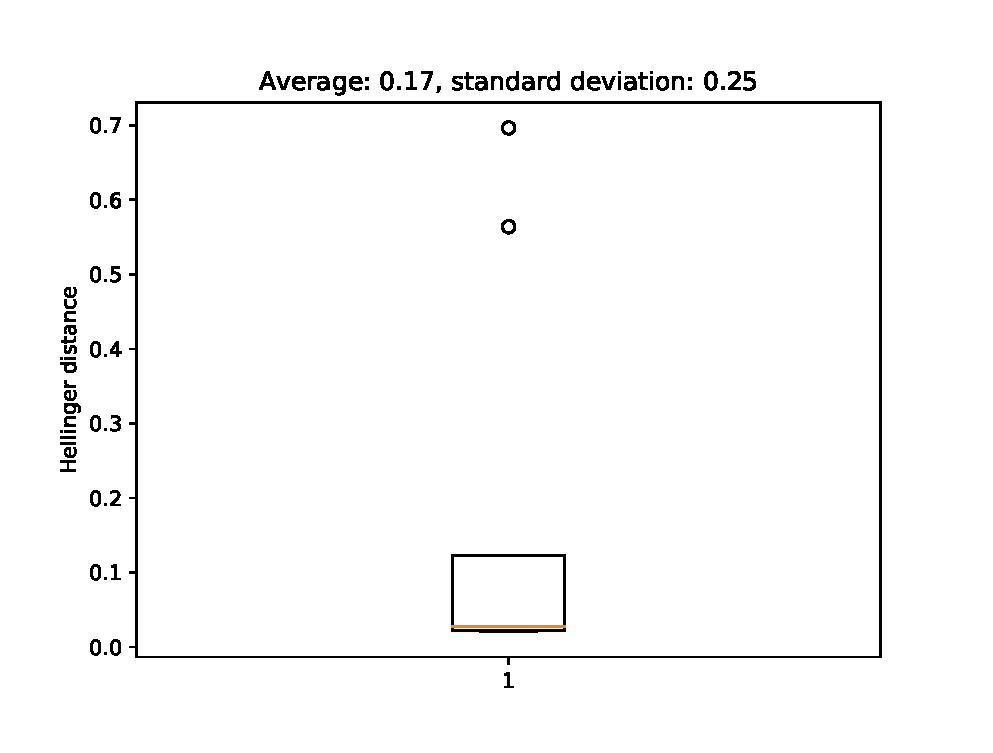
\includegraphics[width=0.5\textwidth]{images/threshold-50.eps}}%
    \subfigure{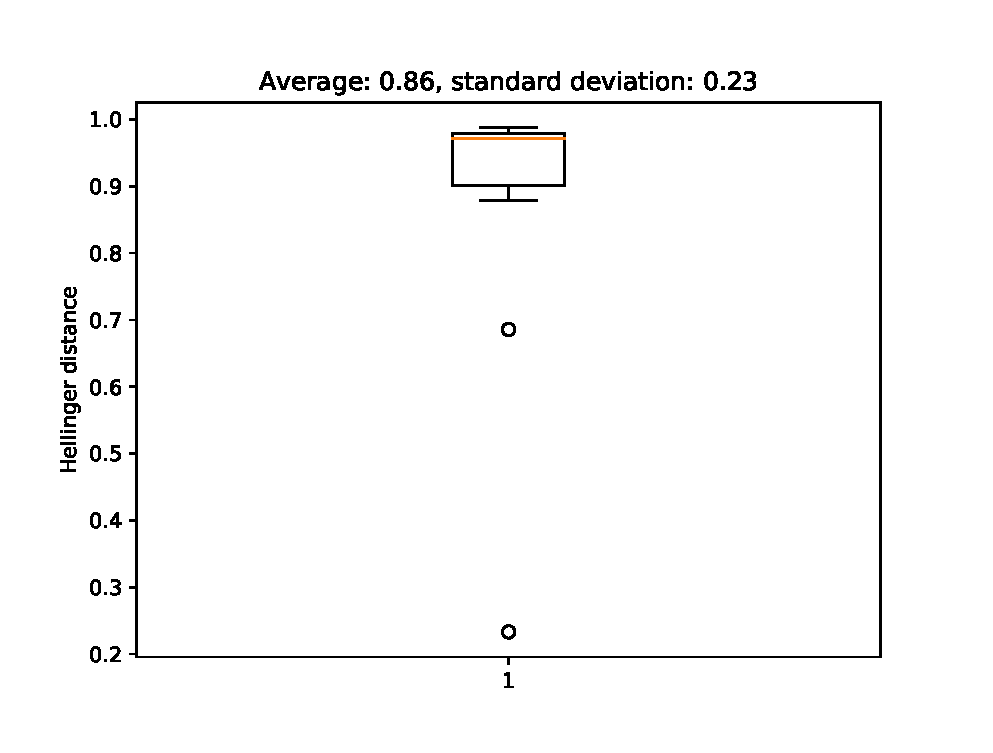
\includegraphics[width=0.5\textwidth]{images/threshold-full.eps}}
    \caption{Boxplot of the computed thresholds for the filtered version (left) and the unfiltered one (right).}
    \label{fig:threshold-box}
\end{figure}

\section{Data exploration} \label{dataexp}
We then compared the structure of the website built through hyperlinks and the inferred networks. 
In this scenario, each link tag is considered an undirected and unweighted edge 
between the URL of the webpage in which it is found and the URL of its \say{href} attribute.

The following proprieties were analyzed:
\begin{itemize}
    \item the degree distribution
    \item the clustering coefficient
\end{itemize}
where the clustering coefficient of a node is the number of possible triangles through that node normalized 
by the potential maximum number of them 
and the average clustering coefficient is just an average between all nodes of a graph.
The histograms of the two proprieties expressed before can be seen in Figure \ref{fig:exploration}. 

Thanks to this analysis we concluded that the inferred networks and the website structure 
are graphs with different characteristics. 
In particular, the structure is sparser and less clustered than the inferred networks.

\begin{figure}[ht]
    \centering
    \subfigure{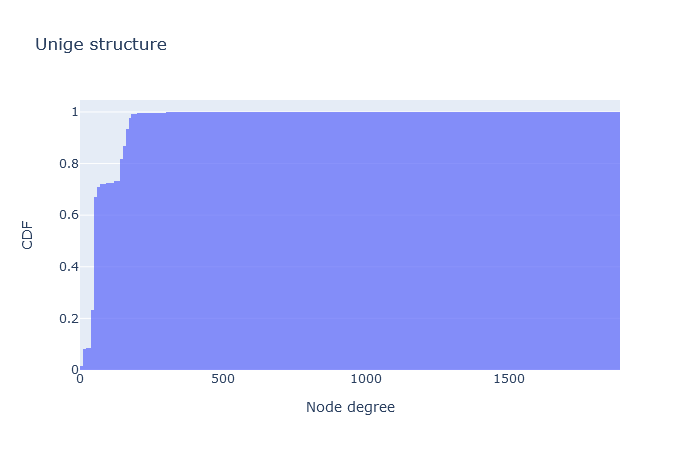
\includegraphics[width=0.5\textwidth]{images/data-exploration/dd/structure.png}}%
    \subfigure{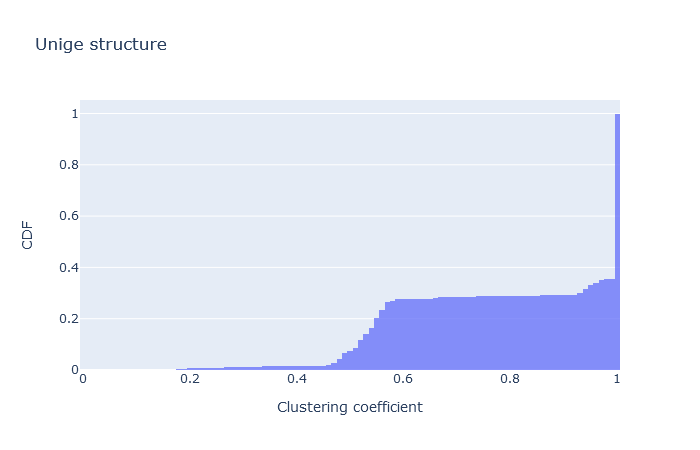
\includegraphics[width=0.5\textwidth]{images/data-exploration/cc/structure.png}}
    \subfigure{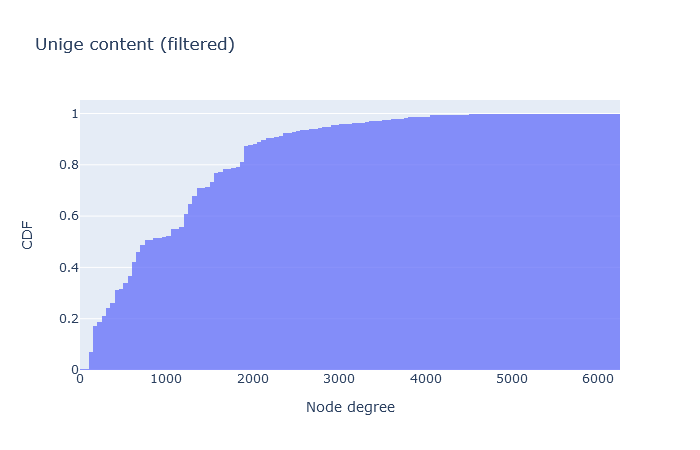
\includegraphics[width=0.5\textwidth]{images/data-exploration/dd/content-filtered.png}}%
    \subfigure{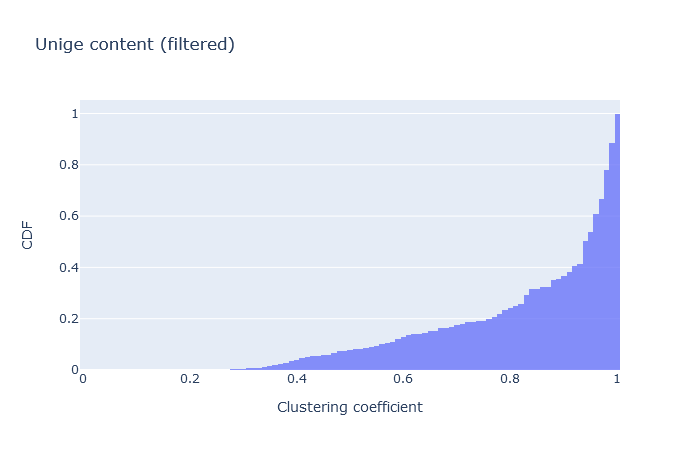
\includegraphics[width=0.5\textwidth]{images/data-exploration/cc/content-filtered.png}}
    \subfigure{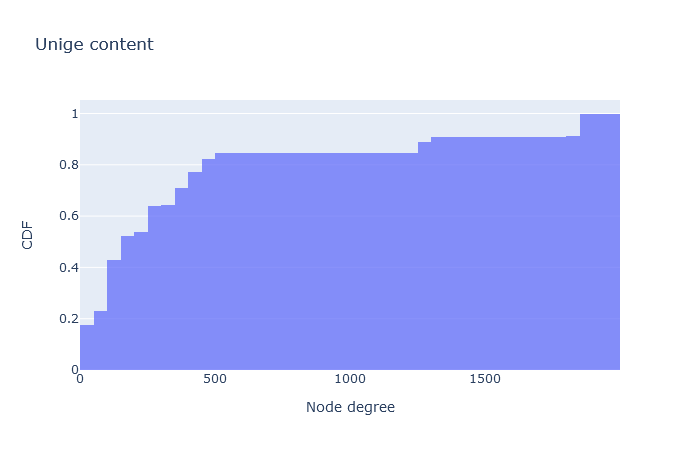
\includegraphics[width=0.5\textwidth]{images/data-exploration/dd/content-full.png}}%
    \subfigure{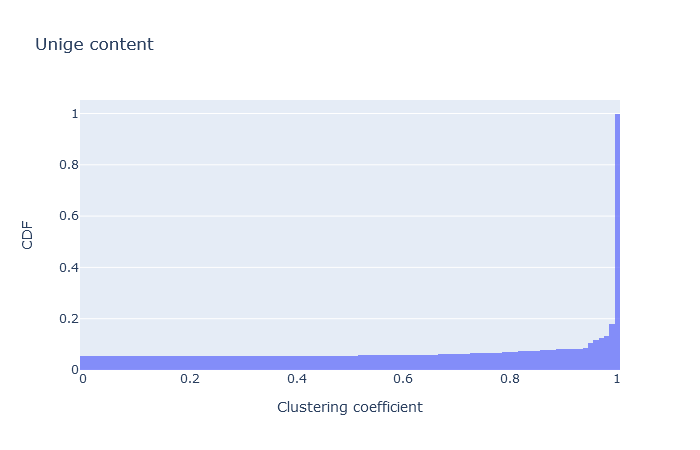
\includegraphics[width=0.5\textwidth]{images/data-exploration/cc/content-full.png}}
    \caption{Cumulative distribution function of the node degrees (first column) 
    and the clustering coefficients (second column).
    The first row is referring to the structure of the website, while
    the second and third row show the results respectively from the filtered similarity graph and the unfiltered one.}
    \label{fig:exploration}
\end{figure}



\section{Evaluation of the results} \label{eval}

Evaluating the quality of the result is not a trivial task. 

Since we knew from Section \ref{dataexp} that the inferred networks are sparse, 
we focused our analysis only on the links between documents. 

Thanks to the prior knowledge of the structure of the UniGe website, we knew that 
all courses provided by UniGe have a particular starting page and that
they share a common tree-like structure. 
For instance, all courses have a page called "Orientamento" which have similar content everywhere. 
Figure \ref{fig:unige-structure} shows this pattern graphically.

In order to provide a score for evaluating if the inferred networks have a meaningful structure, 
we grouped pages by their similarities (e.g. all "Orientamento" webpages are in the same group) and 
we checked how many pages in the group are connected. 

The results show that the unfiltered network recovers more than the 82\% of the edges, 
while the filtered one identifies more than the 99\% of them. 

\begin{figure}[H]
    \centering
    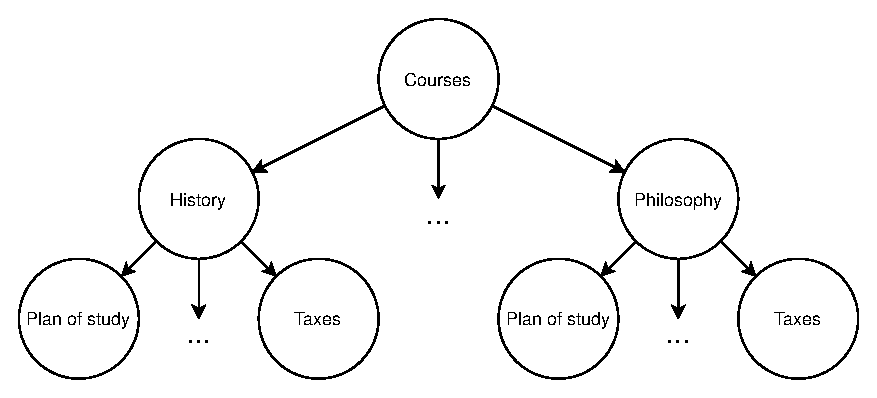
\includegraphics[width=0.5\textwidth]{images/unige-structure.eps}
    \caption{Subsampling of the UniGe website structure with titles translated to English.}
    \label{fig:unige-structure}
\end{figure}



\section{Scaling issues} \label{scaling}

All source code is licensed under the GNU General Public License v3.0 and it can be found at \url{https://github.com/Davide95/msc_thesis/tree/master/code}.
It is written in Python 3.7 and the external libraries used are reported in the relative \texttt{requirements.txt} file.
The source code was also analyzed with \say{flake8} and \say{pylint} to improve readability and to spot bugs.

During the writing of the source code, we encountered some scalability issues related to
the size of the datasets and the computational complexity of the algorithms used.
This section contains a summary of the main strategies used to overcome this
problem. All experiments were tested on a PowerEdge T630 server with the following characteristics:
\begin{itemize}
    \item Intel(R) Xeon(R) CPU E5-2630 v3 @ 2.40GHz (2 sockets)
    \item 8x16GiB of RAM
\end{itemize}

\subsection{NumPy}
The majority of operations in our source code are applied to vectors and matrices.
Modern CPUs provide SIMD (Single Instruction, Multiple Data) instructions like
Intel\textsuperscript{®} AVX-512 to speed up this kind of computations.
In order to use them in the source code, we make use of a library called NumPy\footnote{\url{https://numpy.org/}}
which is interoperable between different hardware and computing platforms.

Furthermore, it allows us to have more numerical stability when dealing with huge
matrices and vectors since it takes into account the limitations
related to storing real numbers using finite-precision floating-point representations
(for instance, using pairwise summation in its source code at
\href{https://github.com/numpy/numpy/blob/v1.18.1/numpy/core/src/umath/loops.c.src}{numpy/core/src/umath/loops.c.src}).

The interested reader can find more advantages of using NumPy reading \cite{5725236}.

\subsection{Numba}
When vectorization is not enough due to the computational costs of the algorithms used, we
compile portions of the Python code to machine code through Numba\footnote{\url{https://numba.pydata.org/}}.

Thanks to this tool, portions of the software can:
\begin{itemize}
    \item run at native machine code speed
    \item run without the involvement of the Python interpreter
    \item be parallelized using multithreading
\end{itemize}
In particular, parallelization is done releasing first the GIL (Global Interpreter Lock).
The interested reader can find more details about it
at \url{https://docs.python.org/3/glossary.html\#term-global-interpreter-lock}.

A basic introduction to how Numba works can be found at \cite{10.1145/2833157.2833162}.

\subsection{Multiprocessing}
We are not able to use NumPy nor Numba where the code is not numerically orientated.
Furthermore, it is not possible to release the GIL in some portions of the code
due to the limitations of the imported libraries.
For these reasons, there are situations in which multiprocessing is used.

In particular, we have to use multiprocessing instead of multithreading during the parsing of
HTML documents explained in Section \ref{sgexp}.
This choice allows us to scale using every core of our machine
but at the cost of increasing the memory consumption of the application.
To have a trade-off between computational costs
and memory issues, we decided to add two parameters that can be tweaked.

\subsection{Optimizing memory usage}
In Python, it is not possible to deallocate manually memory blocks; a GC (Garbage Collector)
is instead responsible to remove data from memory when needed.

To help its work, we try to avoid using the Jupyter Notebook when we found high memory usage.
The reason is mainly that it tends to abuse the use of the global scope for storing variables
and it keeps additional references to objects. Furthermore, we split the code into different steps,
each step restrained in a function.
Between each step, we manually force the GC to collect unused resources.

Finally, we avoid using lists when they do not have a fixed size.
The reason is that frequent append operations in a short time lead in multiple reallocations of
memory which could not be deallocated in time and a memory shortage might happen.
In particular, the problem is that lists in Python are not linked lists but they use
exponential over-allocation every time they lack space. To make a comparison, they have the same
mechanism as ArrayList in Java.
For a more detailed explanation of how memory management works for lists in Python, please refer to
its source code at
\href{https://github.com/python/cpython/blob/3.7/Objects/listobject.c}{Objects/listobject.c}.
